
%(BEGIN_QUESTION)
% Copyright 2010, Tony R. Kuphaldt, released under the Creative Commons Attribution License (v 1.0)
% This means you may do almost anything with this work of mine, so long as you give me proper credit

An electrician wires a reversing motor control circuit as follows:

$$\includegraphics[width=15.5cm]{i03499x01.eps}$$

A wiser electrician warns the one who wired it that it is wrong to have multiple overload heater assemblies in a reversing motor control circuit.  For one motor, he says, there should be only one overload heater block.  The first electrician ignores the second one's advice, and puts this reversing motor control system in service.

Several months later, the motor fails from overheating, despite the overload heater elements being properly sized for this motor.  Explain how it is possible for the motor to overheat in this system.

\vskip 20pt \vbox{\hrule \hbox{\strut \vrule{} {\bf Suggestions for Socratic discussion} \vrule} \hrule}

\begin{itemize}
\item{} How would {\it you} have chosen to communicate the flaw to the first electrician so that your advice would be better heeded?
\item{} What is the proper way to wire a single thermal overload heater in a reversing motor control circuit so that the motor gets the protection it needs?
\item{} What sort of operating scenario might stress this particular (mis-wired) motor more than others, given the improper overload heater installation?
\end{itemize}

\underbar{file i03499}
%(END_QUESTION)





%(BEGIN_ANSWER)

The concept to bear in mind here is that overload heaters function to protect the motor by serving as thermal models of the motor.  As such, they must carry current at all times the motor is carrying current, in order to heat up and cool down along with the motor.  

With {\it two} overload heater assemblies in this circuit (one for each direction), only one of these OL heater assemblies will heat at any given time the motor is running.  If the motor switches direction, current will now pass through the ``cold'' heater while the ``warm'' heater cools off, despite the fact the motor itself continues to remain warm from use.

\vskip 10pt

If the motor is run hard in one direction, then reversed, the ``cold'' overload heater assembly will not accurately reflect the pre-heated status of the motor.  This may lead to a condition of overload, where the motor is allowed to heat up too much because the too-cold OL heaters haven't been heating as long as the motor has.

%(END_ANSWER)





%(BEGIN_NOTES)


%INDEX% Electronics review: AC motor control circuit

%(END_NOTES)

